\begin{frame}
\frametitle{Thrombolysis (\emph{'Clot-busting'} medication) in stroke}

While the clot is still fresh, thrombolysis may be given to help break down the clot and restore blood flow.

\vspace{3mm}

\begin{center}
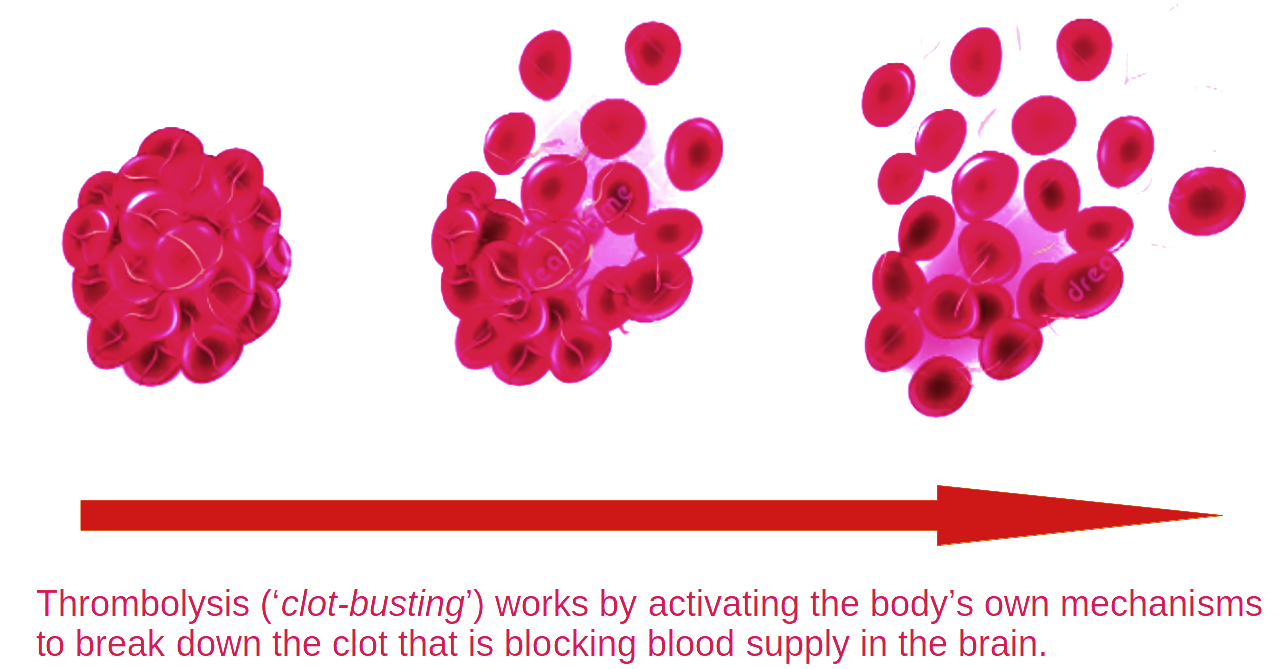
\includegraphics[width=0.70\textwidth]{./images/thrombolysis_mechanism}
\end{center}

\textbf{Drawbacks/limitations}: There is a risk of severe bleed (in about 1 in 50 patients on average, with risk increasing with stroke severity), and thrombolysis loses effectiveness over about the first 5-6 hours.

\end{frame}